\chapterhead{5}{Keeping a Running Total}{Adding up what is lost at every step}\label{ch5}

A bouncing ball loses some of its lift on every bounce. To follow the energy, write the height of each bounce and keep a \textbf{running total} of what has been lost so far. The running total grows. The height left plus the total lost always adds back to the start.

\begin{center}
\sffamily\small\renewcommand{\arraystretch}{1.5}
\begin{tabular}{@{}p{3.4cm}p{3.7cm}p{3.7cm}@{}}
\toprule
\textbf{Model} & \textbf{What it keeps} & \textbf{What it drops}\\
\midrule
A bounce list & the height after each bounce & the sound of each thud\\
A running total & the loss so far & what each loss became\\
A final check & height left $+$ lost $=$ start & small errors in reading\\
\bottomrule
\end{tabular}
\end{center}

\begin{tryit}{Bounce by bounce}
Drop the ball from 40~cm. A helper writes down the top height of bounces 1, 2, 3 and 4 (a phone video helps). Work out the loss at each bounce and the running total.\par\medskip
\renewcommand{\arraystretch}{1.6}
\begin{tabular}{|l|c|c|c|c|}
\hline
\textbf{Bounce} & \textbf{Height} & \textbf{Lost this bounce} & \textbf{Lost so far} & \textbf{Height + lost}\\ \hline
Start & 40 & 0 & 0 & 40\\ \hline
1 & & & & \\ \hline
2 & & & & \\ \hline
3 & & & & \\ \hline
4 & & & & \\ \hline
\end{tabular}
\end{tryit}

\begin{worked}{Practice numbers, not from a real test}
Heights: 28, 20, 14, 10.\\
Lost at each bounce: $40-28=12$, $28-20=8$, $20-14=6$, $14-10=4$.\\
Running total lost: 12, then $12+8=20$, then $20+6=26$, then $26+4=30$.\\
Check: $10+30=40$. The account balances.
\end{worked}

\begin{center}
\sffamily\small\renewcommand{\arraystretch}{1.5}
\begin{tabular}{@{}lrrrr@{}}
\toprule
\textbf{Bounce} & \textbf{Height} & \textbf{Lost now} & \textbf{Lost so far} & \textbf{Check}\\
\midrule
Start & 40 & 0 & 0 & 40\\
1 & 28 & 12 & 12 & 40\\
2 & 20 & 8 & 20 & 40\\
3 & 14 & 6 & 26 & 40\\
4 & 10 & 4 & 30 & 40\\
\bottomrule
\end{tabular}
\end{center}

\begin{multix}[hmm]\multixbot[hmm]\tcblower
After bounce 3 I lost only 6 units, so the total lost is 6. Earlier bounces are history and do not count. Right?
\end{multix}

\trust{We wrote every bounce, and after each one we added the height left to the total lost and checked that it came back to the start.}
{Every row gave 40, so no unit was dropped from the account.}
{What each loss turned into. A running total says how much, not into what.}

\begin{keepbox}
We turned a bouncing ball into a table. \textbf{We kept} \wline[3.4cm] \textbf{and we set aside} \wline[3.4cm].
\end{keepbox}

\clearpage

\begin{tryit}{On a rug}
Repeat on a rug, with the drop at 40~cm.\par\medskip
\renewcommand{\arraystretch}{1.6}
\begin{tabular}{|l|c|c|c|c|}
\hline
\textbf{Bounce} & \textbf{Height} & \textbf{Lost this bounce} & \textbf{Lost so far} & \textbf{Height + lost}\\ \hline
1 & & & & \\ \hline
2 & & & & \\ \hline
3 & & & & \\ \hline
\end{tabular}
\end{tryit}

\begin{worked}{Practice numbers}
Rug heights: 14, 5, 2. Lost: 26, 9, 3. Running total: 26, 35, 38. Check $2+38=40$.\\
The rug took 26 units at the first bounce, against 12 on the floor.
\end{worked}

\clearpage

\begin{puzzle}{Running total}
Bounces from a 40 drop: 30, 22, 16. Lost each time \wline[1.2cm], \wline[1.2cm], \wline[1.2cm]. Total lost \wline[1.2cm]. Check: $16+$ total $=$ \wline[1.2cm]
\end{puzzle}

\begin{puzzle}{Fill the table}
Start 50. Bounces 36, 26, 18. Lost so far after each bounce: \wline[1.2cm], \wline[1.2cm], \wline[1.2cm].
\end{puzzle}

\begin{puzzle}{Biggest loss}
Lost this bounce were 12, 8, 6, 4. Which bounce lost the most? \wline[1.6cm] Why might it lose most? \wline[4cm]
\end{puzzle}

\begin{puzzle}{Add the losses}
Add 12, 8, 6 and 4. \wline[1.6cm]
\end{puzzle}

\begin{puzzle}{Fix the total}
A student wrote the total lost after bounce 3 as 6. What is the right number? \wline[1.6cm]
\end{puzzle}

\clearpage

\begin{puzzle}{Chain of steps}
Start 60. Steps lose 10, 9 and 7. How many are left? \wline[1.6cm]
\end{puzzle}

\begin{puzzle}{Where did it go?}
Name two places a ball's lost energy goes at each bounce. \wline[5cm]
\end{puzzle}

\begin{puzzle}{Draw the chain}
Draw circles for a start of 40, a bounce of 28 and a second bounce of 20, with the loss at each step as its own circle.
\begin{center}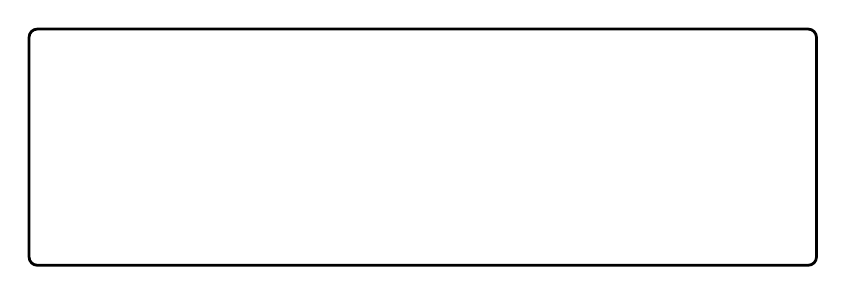
\begin{tikzpicture}\draw[line width=1pt,rounded corners=3pt] (0,0) rectangle (10,3); \end{tikzpicture}\end{center}
\end{puzzle}

\begin{puzzle}{Wrap}
A student wrote ``The ball ran out of energy.'' Wrap it with a better claim. \wline[6cm]
\end{puzzle}

\begin{puzzle}{Link}
A running total is like a savings jar. Say what you add each time and what you check at the end. \wline[6cm]
\end{puzzle}
\clearpage

\thispagestyle{fancy}
\subhead{Bounce ledger}
Make a full ledger for a floor of your choice, from a 40~cm drop.\par\medskip
\renewcommand{\arraystretch}{2.8}
\begin{tabularx}{\linewidth}{|>{\sffamily\small\bfseries}p{2.2cm}|X|X|X|X|}
\hline
Bounce & Height & Lost now & Lost so far & Height + lost \\ \hline
1 & & & & \\ \hline
2 & & & & \\ \hline
3 & & & & \\ \hline
4 & & & & \\ \hline
5 & & & & \\ \hline
\end{tabularx}

\vspace{8pt}
Does every row come back to 40? \wline[7cm]\\[10pt]
Which row has the biggest loss? \wline[5cm]\\[10pt]
Draw your running total as a bar chart.\par\medskip
\begin{tikzpicture}\draw[ink!70,line width=1pt,rounded corners=3pt] (0,0) rectangle (11.4,4.4);\end{tikzpicture}
\clearpage
